\documentclass[../main.tex]{subfiles}

\begin{document}
\section{Capillary discharge, Jitter}\label{sec:jitter}
Experiments in which plasma channels are supposed to be ready-to-use guiding media require a low ignition jitter (the spread in initiation of the current), so as to provide results reproducible on shot-to-shot basis. Typical guiding window lasts about \SIrange{50}{100}{\ns}, so ignition jitter of about \SI{10}{ns} would be tolerable.

This was our goal as a first experiment with the gas injected capillaries.

% A schematic drawing of the system is shown in figure \ref{fig:scheme}.
\begin{marginfigure}
    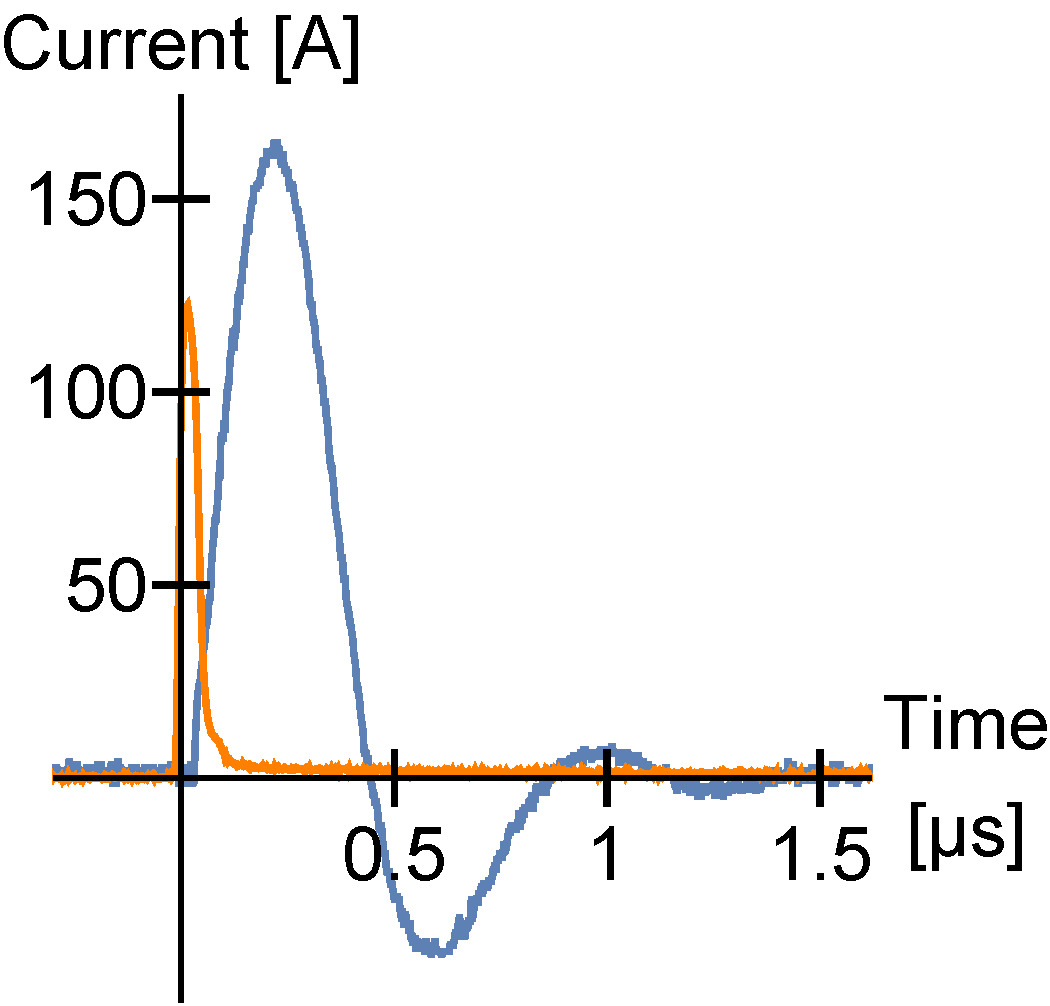
\includegraphics[width=\marginparwidth]{figures/jitter/discharge_sample.pdf}
    \caption{A typical plasma discharge. Blue waveform is the current profile obtained from the Rogowsky coil. In green is the photo--detector rise up from the igniting Nd:Yag pulse.}
    \label{fig:discharge_sample}
\end{marginfigure}
To anchor the discharge starting process to a fixed event to which we can refer, we mounted a photo--detector close to the igniting laser radiation output, thus enabling one to fix a time event at which the plasma discharge occurs; The photo--detector allows for visualizing the synchronization. Recording to an oscilloscope both the photo--diode rise-up signal and the current profile obtained from the Rogowsky coil, we monitored the igniting pulse and the discharge current for consecutive 12 ignitions performed at constant time intervals.
\begin{figure}
    \centering
    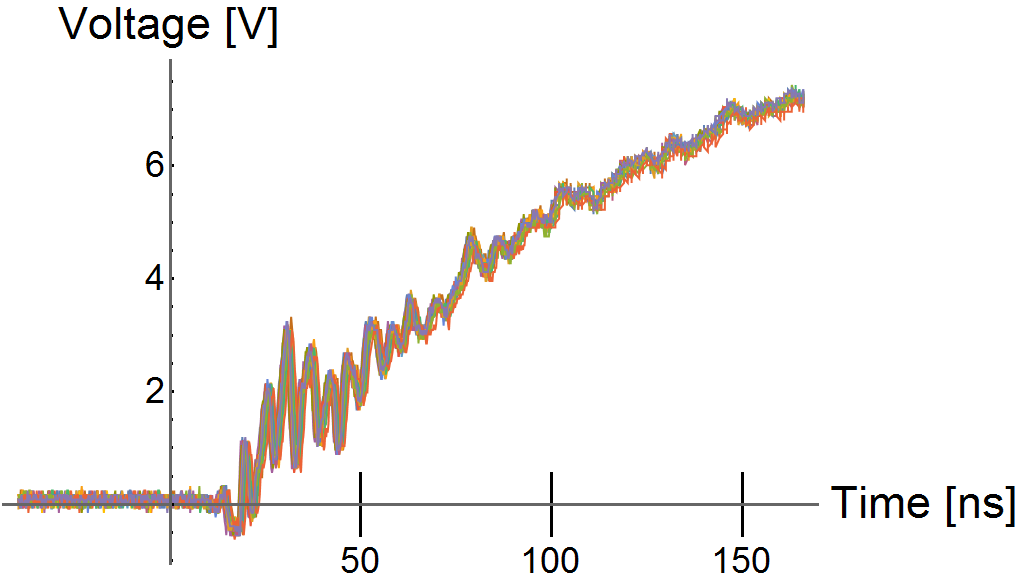
\includegraphics[width=\textwidth]{figures/jitter/low_jitter.png}
    \caption{12 consecutive capillary discharges recorded one on top of the other, demonstrating low ignition jitter when generating plasma in the capillary.}
    \label{fig:low_jitter}
\end{figure}

The time resolution is evaluated while taking into consideration both the oscilloscope sampling rate and the prior to ignition electrical components' jitter. The jitter is calculated as half the difference between the earliest and latest ignition timing of multiple independent ignitions. Overall, we evaluate the jitter to be
\begin{equation}
	\tau_\text{jitter}\approx 6\pm 1\si{\ns}
\end{equation}
This implies that we can determine the time window for optical guiding, with no concerns of shooting too early or too late with respect to the over-all plasma lifetime. Also, we deduce that our system and its over all components is relatively stable and reliable.

On the contrary, a much less stable regime was observed if the experiment is repeated \textbf{without} the igniting laser pulse. The explanation is that the electrical breakdown evolves in a much less deterministic behaviour; The process of the electrons being ripped from the molecules in a cascading manner is rather not stable. The jitter observed under this constraint of absent igniting laser pulse is on the order of \SI{80}{\us}. See figure \ref{fig:multiple}.
\begin{figure}
    \centering
    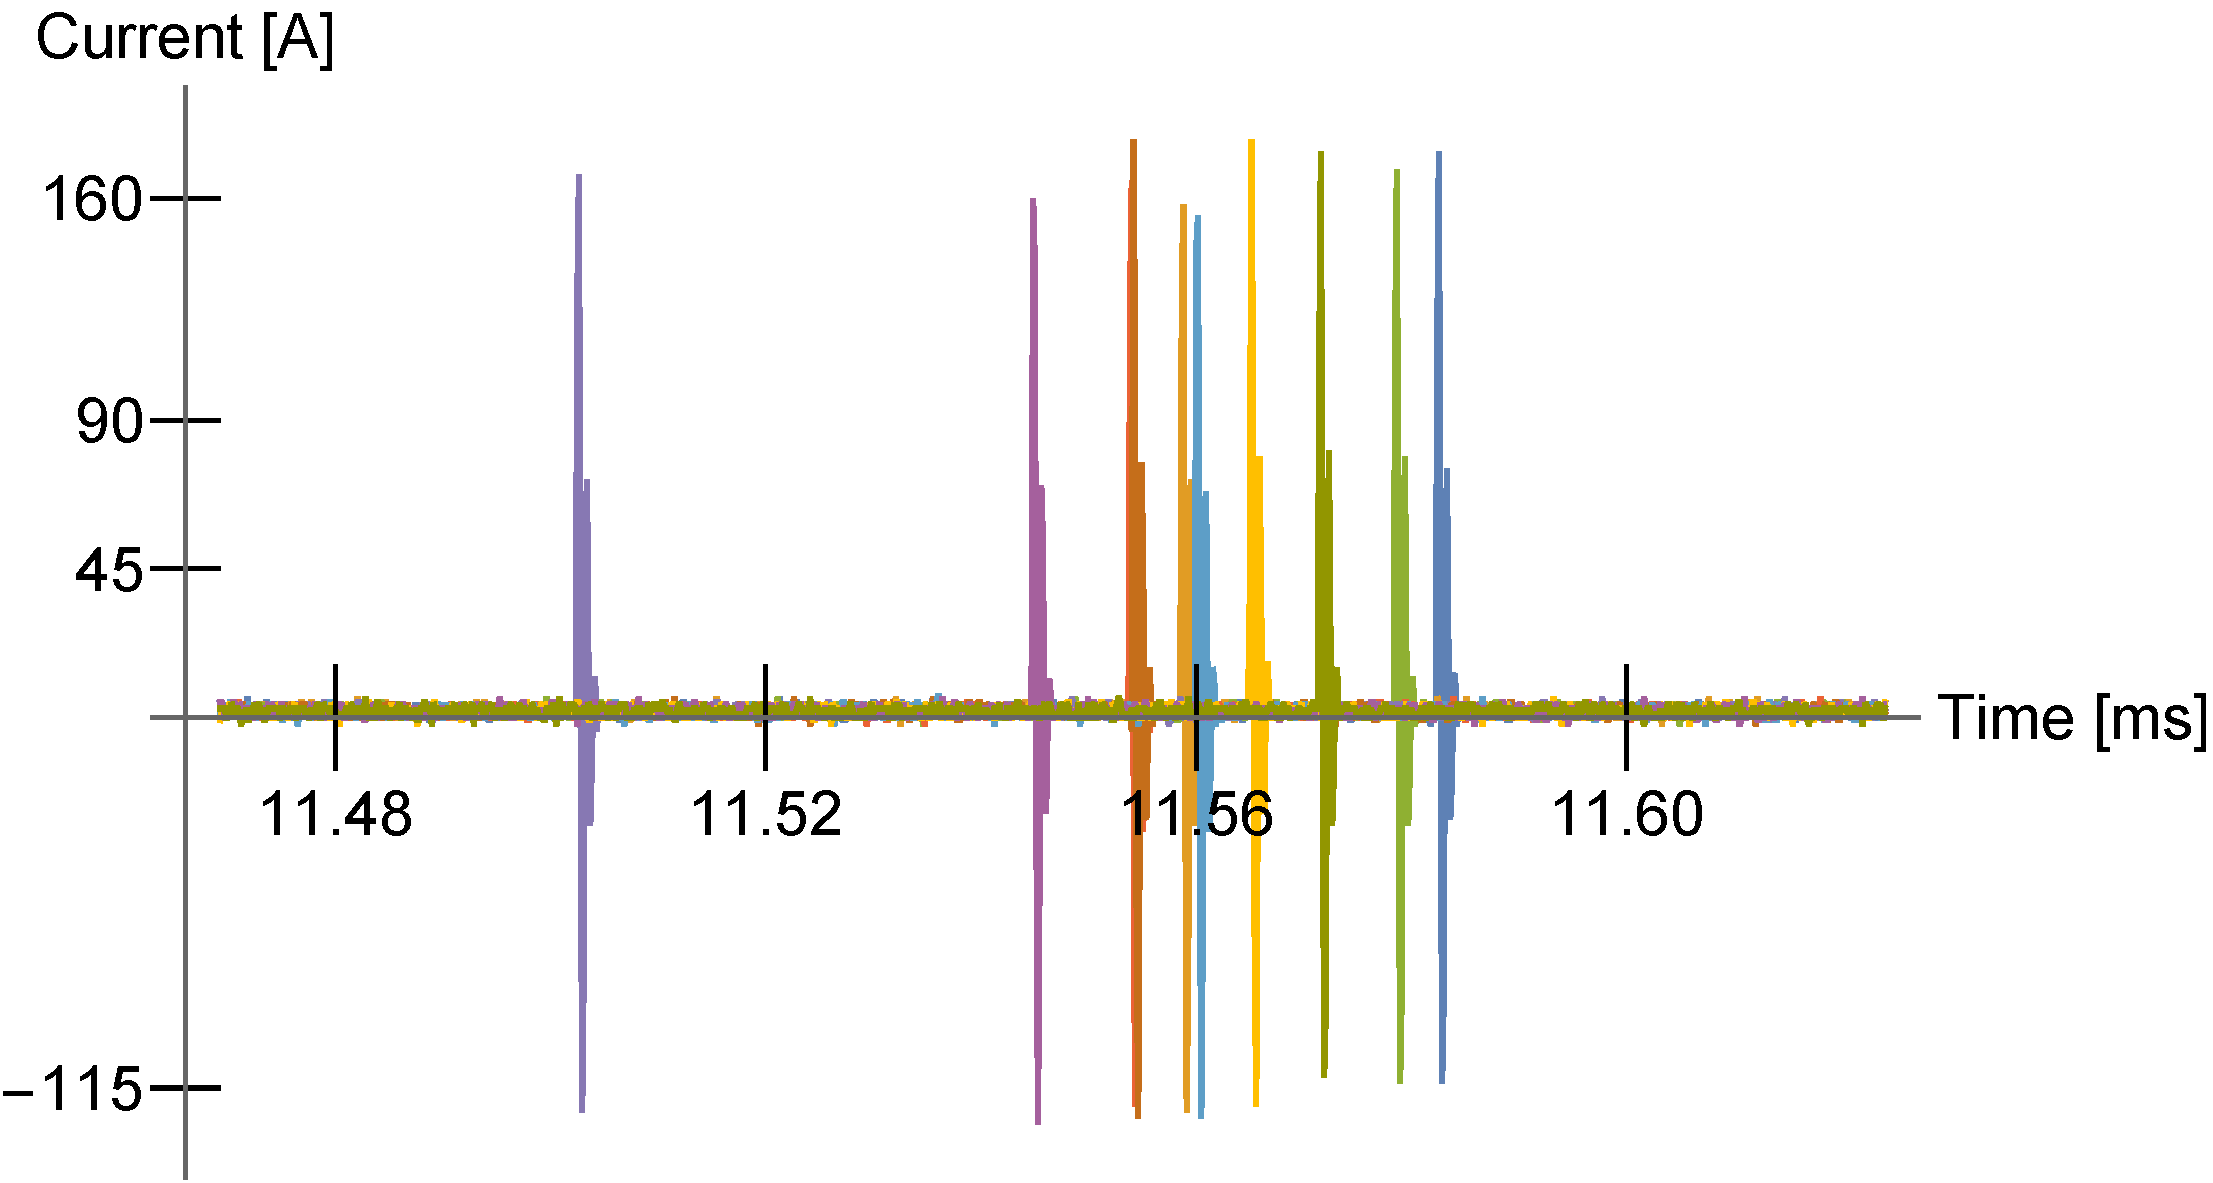
\includegraphics[width=\textwidth]{figures/jitter/multiple.pdf}
    \caption{Nine different plasma discharges without the igniting Nd:Yag laser pulse, all recorded on the same axes. The time segment is zoomed--in in the bottom inset.}
    \label{fig:multiple}
\end{figure}

\section{Duration of the hollow density profile}\label{sec:duration-of-guiding}
We are now in a position to estimate the timing and duration of the hollow density profile. For that, with the system set--up as in the previous measurement, we aligned the \SI{800}{\nm} oscillator laser (\ref{ssec:lasers}) through the capillary and directed the outgoing beam out of the vacuum chamber to the active area of a fast photo-diode detector. This detector output was connected to the same measuring oscilloscope as well.

\begin{figure}
\centering 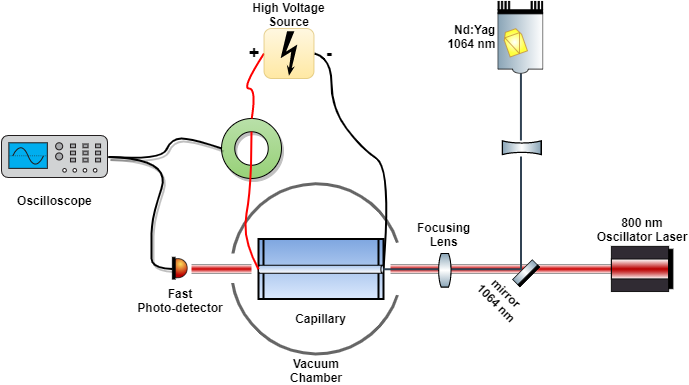
\includegraphics[width=\textwidth]{figures/oscillator.png}
\caption{System set--up used to measure the duration of the plasma channel.}
\label{fig:oscillator}
\end{figure}
Upon plasma discharge, we recorded the optical guiding of the pulse--train, shown in figure \ref{fig:oscillator_single}, and watched after an increase in the detected signal amplitude while it interacts with the plasma inside the capillary. The result is shown in figures \ref{fig:guiding1}-\ref{fig:guiding2}.

The optical guiding is quantitatively estimated as the transmission factor --- ratio of the maximal amplitude obtained during the guiding window to the amplitude before the plasma discharge.

At the upper plot is the plasma discharge current profile, similar to that shown in \ref{fig:discharge_sample}, as delivered from the Rogowsky coil. The applied voltage for these two measurements was $\sim$\SI{7}{\kilo\volt}. Along it is the signal arriving from the Nd:Yag photo--diode detector (green waveform), which, as mentioned before, tells us whether the discharge is timed with the igniting laser and is jitter--controlled. The lower waveform is that recorded from the fast--photodiode with the oscillator laser as its signal source.
\begin{figure*}
    \centering
    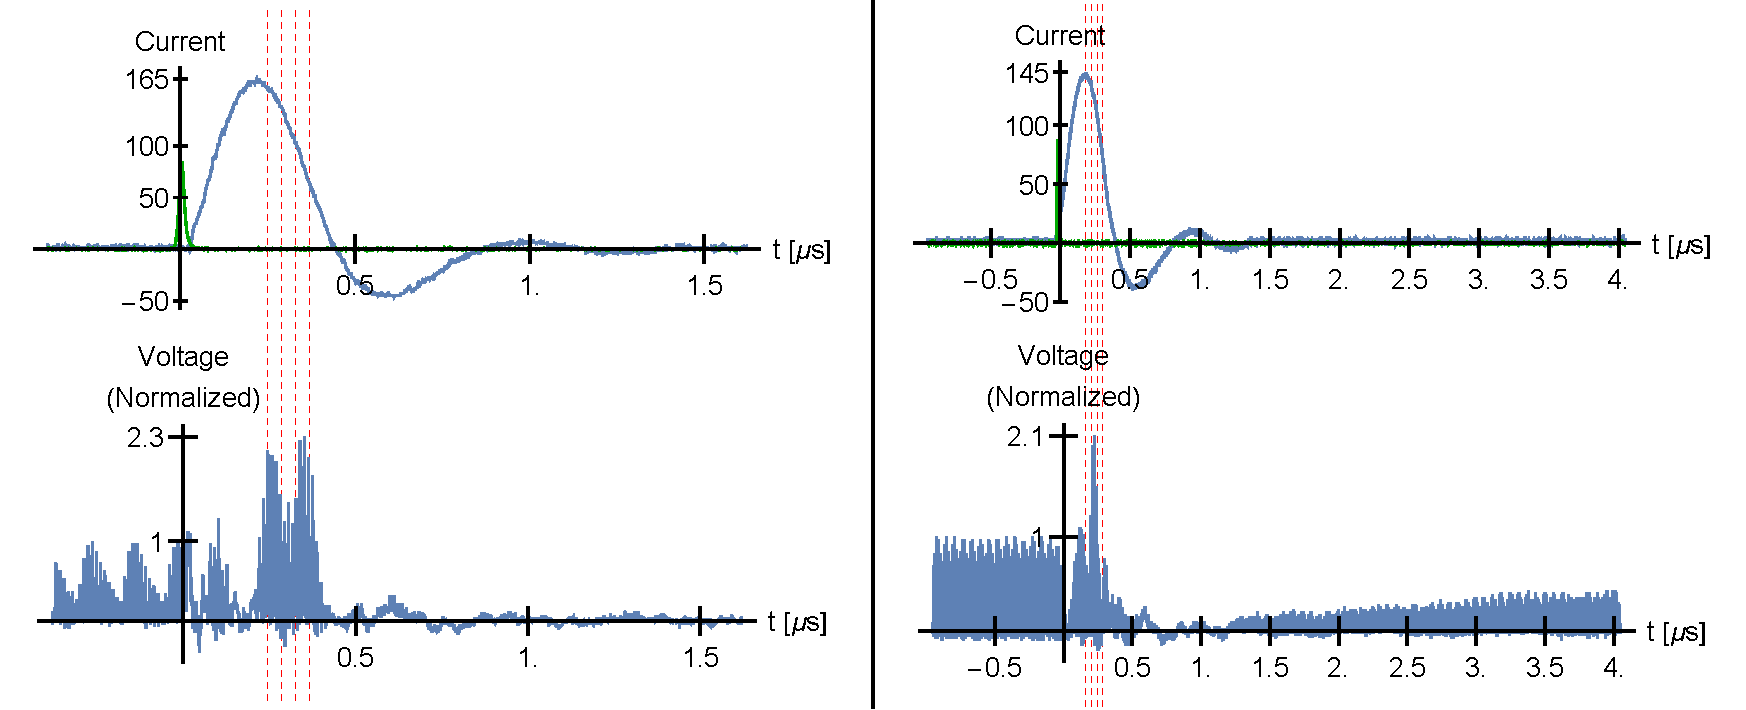
\includegraphics[width=\textwidth]{figures/oscillator/guiding1.pdf}
    \caption{Guiding of the pulse train (bottom) shown in reference to the igniting laser (\textcolor{ForestGreen}{green}, top), and the discharge current.}
    \label{fig:guiding1}
\end{figure*}
\begin{figure}
    \centering
    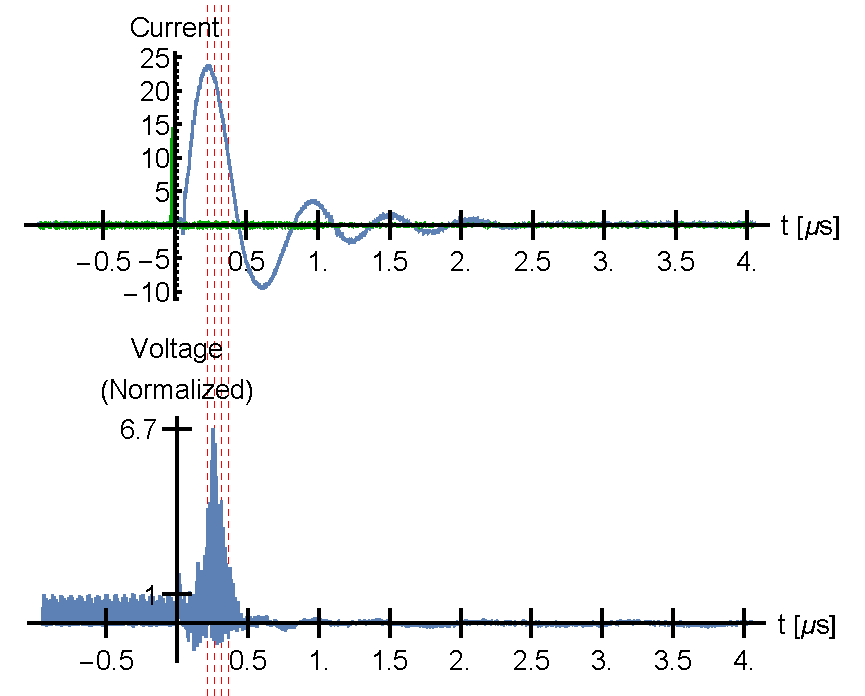
\includegraphics[width=\textwidth]{figures/oscillator/guiding2.pdf}
    \caption{Guiding of the oscillator laser, with a higher voltage difference applied to the capillary electrodes, $\sim$\SI{10}{\kilo\volt}, giving a larger transmission factor.}
    \label{fig:guiding2}
\end{figure}

The explanation for the improved transmission of the laser radiation during the formation of the plasma channel was mentioned in section \ref{ssec:plasma-waveguides}: If an inverted radial density profile (minimum on the axis, refer to figure \ref{fig:rdp_parabola}) can be created, a plasma lens forms and the radiation is focused and trapped by the plasma. See figure \ref{fig:chen4_31}.
\begin{marginfigure}
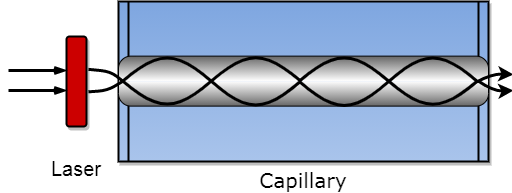
\includegraphics[width=\marginparwidth]{figures/chen4_31.png}
\caption{Plasma confined inside the capillary will trap the \SI{800}{\nm} laser light only if the plasma has a density minimum on axis.}
\label{fig:chen4_31}
\end{marginfigure}

An additional phenomenon to remark is that the oscillator pulse--train is blocked by the plasma in the later stage of the discharge. In this part of the plasma lifetime the capillary wave--guide is not operating. The plasma functions as a medium that refracts the radiation in some uncontrolled way to the capillary plastic walls, thus less light is collected by the photo--detector. The system approaches the state prior to the ignition after the plasma is diffused into the vacuum chamber.

In addition to the timing and duration of the plasma channel, we measured the optical guiding for different parameters: applied voltage over the capillary electrodes, laser power and injected gas pressure. Analysis shows that the stronger parameter is the applied voltage. The effect is seen in figure \ref{fig:guiding2}, for which a $\sim$\SI{11}{\kilo\volt} was applied to the capillary terminals, and a peak current of \SI{240}{\A} was measured by the Rogowsky coil. The optical guiding for this measurement is as high as $\sim 6.7$.

\begin{figure}
    \centering
    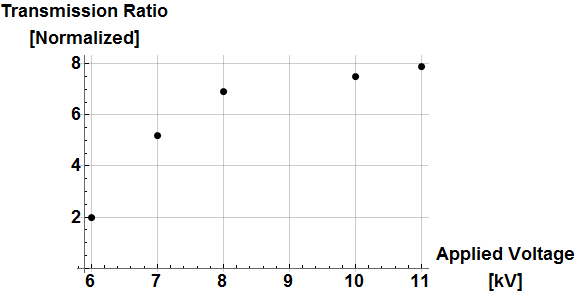
\includegraphics[width=\textwidth]{figures/oscillator/voltage vs guiding.png}
    \caption{Correlation for optical guiding to different applied voltage differences across the capillary ends. This behaviour suggests an upper limit to the transmission ratio.}
    \label{fig:voltagevsguiding}
\end{figure}

The $\sim$ \SI{12.5}{\ns} time resolution of the pulse--train enables us to estimate the temporal duration of the plasma channel (the vertical red grid lines in figures \ref{fig:guiding1}-\ref{fig:guiding2} as a visual aid) to be $$\Delta t_\text{channel}=\SIrange{50}{100}{\ns}.$$.

\section{Spectroscopic measurements}\label{sec:spectro}
To estimate quantitatively the depth of the plasma channel and the plasma density, we performed an additional measurement with a spectrometer and a fast camera, introduced in section \ref{ssec:spectro}, and analysed the emission line attributable to Stark effect.

\subsection{Radial density profile}\label{ssec:radial}
We installed an imaging system that images the capillary entrance, as shown in figure \ref{fig:radial_system}. For an accurate and reliable measurement, we needed to over--come two main difficulties:

\begin{figure}
\centering
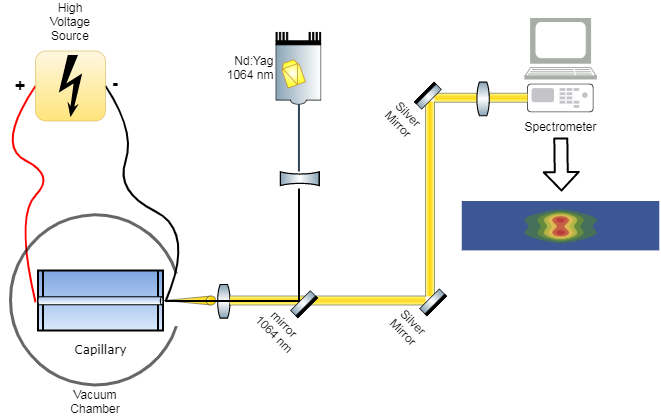
\includegraphics[width=\textwidth]{./figures/spectro/radial_system.png}
\caption{Experimental setup and typical spectrum of the plasma at the exit of the capillary.}
\label{fig:radial_system}
\end{figure}

In order to magnify the circular cone of plasma light emitted from the capillary entrance imaged on the spectrometer slit, we placed a converging lens in a distance a bit longer from its focal length so to obtain as large as possible transverse magnification. The drawback is the loss of irradiance, which was compensated with the gain mechanism of the microchannel plate of the CCD camera.

Secondly, as mentioned before (\ref{sec:jitter}), the plasma channel lasts for \SIrange{50}{150}{\ns}, and this leads to a constraint on the duration of the camera gating window. Clearly, a long exposure time ($\gtrsim \SI{1}{\us}$) would yield a constant profile. But to capture the hollow plasma channel we rather gated (using the digital delay generator) the CCD camera to exposure times of \SI{40}{\ns}\marginnote{To produce a sharp image of a moving subject, a fast shutter speed is required.}. That obviously led to signal--to--noise--ratio difficulties when analysing the digital data --- the shutter is not opened for long enough for the image-sensing area to be exposed to light.

The simple imaging system was composed of two converging lens (fused-silica, bi-convex, \diameter 2 inch), the first with a shorter focal length, that imaged the capillary entrance magnified by $\times 5$ on the spectrometer entrance slit. I.e., the image of a \SI{0.5}{\mm} capillary was $\sim$ \SI{2.5}{\mm} in diameter, corresponding to about \SI{40}{\percent} of the CCD's vertical range. The spectrometer slit had the width of \SI{150}{\micro\metre}, providing a spectral resolution of about \SI{0.3}{\nm}.

The grating was rotated to the central wavelength of \SI{656.3}{\nm}, which, as mentioned in section \ref{sec:hydrogen}, is the central wavelength of hydrogen H\textsubscript{$\alpha$} line. This line, when emitted within a plasma, undergoes Stark broadening from which the electron density can be deduced, with the density estimate based on equation \ref{eq:delta_lambda}. A dielectric mirror coated for zero degrees at \SI{1.064}{\um} prevented the radiation of the igniting laser from entering the spectrometer.

We gated the CCD camera, as stated, to \SI{40}{\ns} gate--on time at time windows that correspond to the maximal transmission of the oscillator signal (as described in \ref{sec:duration-of-guiding}), and set the gain of the microchannel plate to its highest, at the level of 9.

The raw spectroscopic images captured by \textit{Andor} in a \texttt{.fit} file format were processed in the \textit{Matlab} environment and its curve-fitting tool. The steps for the analysis are as follows (figure \ref{fig:spectra_analysis}):
\begin{itemize}[label={$-$}]
\item For each row of the data (256 rows), find a Lorentzian fit for the intensity profile, with the line half--width ($\Delta\lambda_{1/2}\left[\text{px}\right]$) as a free parameter (figure \ref{fig:single-lorentzian}).
\item Then, plot the set of $\Delta\lambda_{1/2}$ versus the corresponding spatial coordinate.
\item To convert $\Delta\lambda_{1/2}\left[\text{px}\right]$ to \si{\nm}, we used the known Sodium doublet for the lines $D_1=\SI{589.59}{\nm}$ and $D_2=\SI{589.00}{\nm}$, which corresponds to 18 horizontal pixels.
\item This line broadening was translated to plasma density using equation \ref{eq:delta_lambda}.
\item Finally, convert the spatial coordinate axis to position (capillary radius, \si{\mm}) using the magnification factor of the imaging system together with the pixel--to--\si{\um} conversion factor\sidenote{pixel size = \SI{26}{\um}$\times$ \SI{26}{\um}}.
\end{itemize}

\begin{figure*}
    \centering
    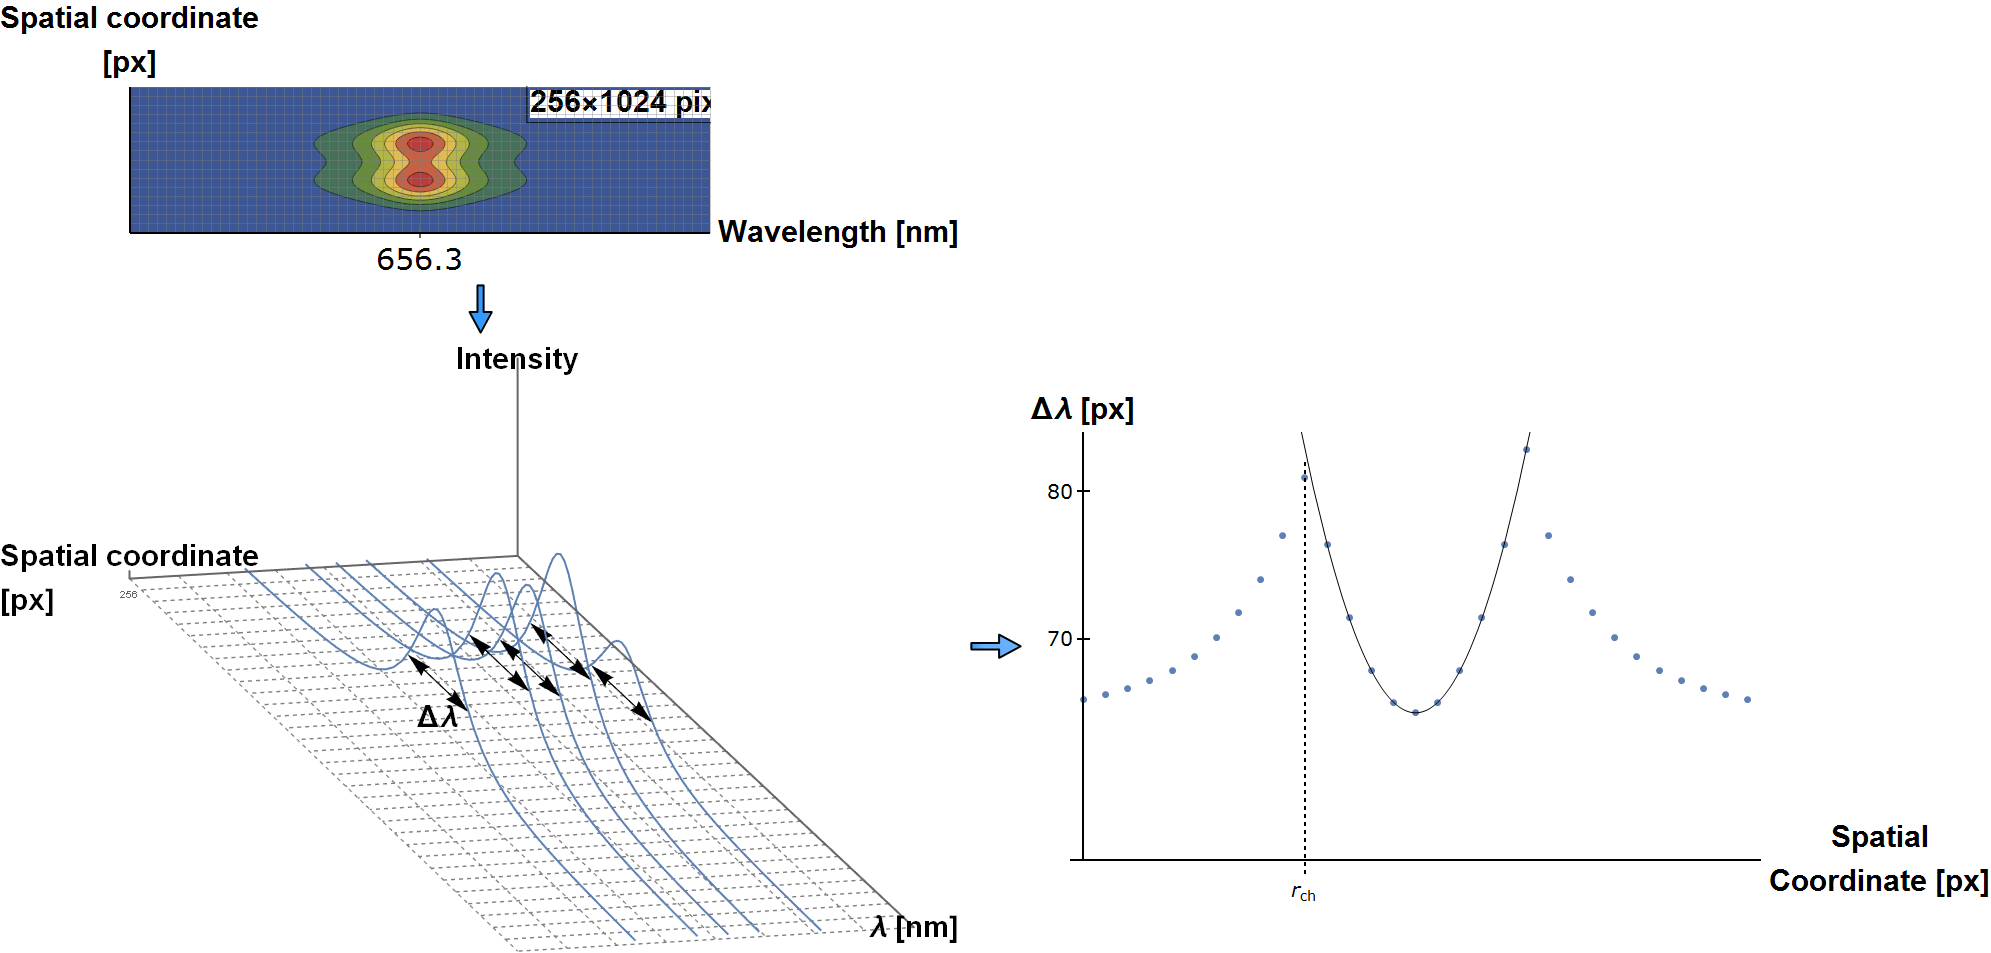
\includegraphics[width=\textwidth]{figures/spectro/spectra_analysis.png}
    \caption{An explanatory figure of the steps involved in the analysis of the raw spectroscopic data.}
    \label{fig:spectra_analysis}
\end{figure*}
\begin{figure}
    \centering
    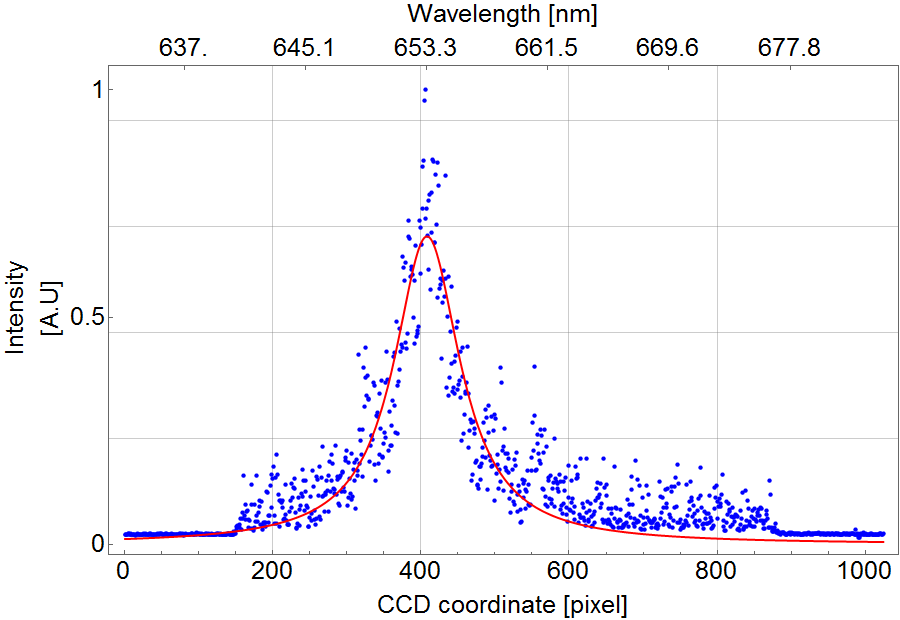
\includegraphics[width=\textwidth]{figures/spectro/sample-lorentzian.png}
    \caption{Stark broadening of the H\textsubscript{$\alpha$} line. In out measurements the broadening was on the order of \SI{3}{\nm}.}
    \label{fig:single-lorentzian}
\end{figure}

Figure \ref{fig:plasma_channel_spectro} plots the experimentally measured plasma density as a function of position (capillary radius) across a \SI{500}{\um} capillary diameter at a delay time \SI{400}{\ns} after the rise of the discharge current pulse. The maximum discharge current was \SI{165}{\A}.

\begin{figure}
\centering
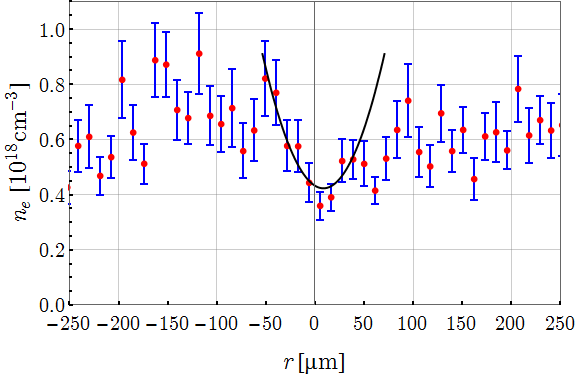
\includegraphics[width=\textwidth]{figures/spectro/parabolic.png}
\caption{Radial density profile of the plasma from the measured spectrum, \SI{400}{\ns} after the rise of the current.}
\label{fig:plasma_channel_spectro}
\end{figure}

For these conditions, there is a density minimum on the axis of the capillary; at early delay times the minimum at the radial density profile was not created, and at later delay times it disappears. The increase in the electron density is found to be 
\begin{equation}
    \Delta N_e \sim \SI{.4e18}{\per\cubic\cm}
\end{equation}

with
\begin{equation}
r_\text{ch}\approx \SI{50}{\um} \text{ and } N_e\left(0\right)\approx \SI{0.4e18}{\per\cubic\cm}.
\end{equation}

These conditions provide an optimal plasma channel that can be used for guiding an intense laser pulse for LWFA accelerators.

\subsection{Longitudinal density profile}\label{ssec:longi}

The method described in section \ref{ssec:radial} allows for measuring the radial density profile only at the capillary output, but it is also important to verify longitudinal homogeneity of the plasma density. For this purpose the entire length of the \SI{5}{\cm} capillary was imaged along the entrance slit of the spectrometer.
\begin{figure}
    \centering
    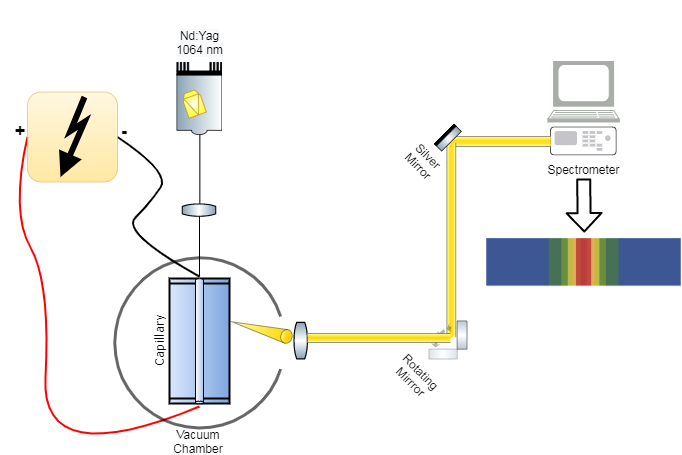
\includegraphics[width=\textwidth]{figures/spectro/longitudinal_system.png}
    \caption{Experimental system to image plasma emission in the longitudinal dimension.}
    \label{fig:longi_system}
\end{figure}

To achieve that, we built the system shown in figure \ref{fig:longi_system}, with the main difference from the one before, figure \ref{fig:radial_system}, being a periscope assembly (not shown) used to flip the strip of plasma emission by \SI{90}{\degree} so it enters into the entrance slit of the spectrometer. As opposed to the magnification issue we had before, now a minification of the image was sought. We positioned the capillary on a move--able mount, and performed 5 capillary discharges, each corresponding to a segment of \SI{1}{\cm} of the capillary length. The plasma density was estimated based on the H\textsubscript{$\alpha$} line Stark broadening, as before; Gate--on time windows of the Andor ccd camera were on the scale of \SI{1}{\us}. The result is shown in figure \ref{fig:longi_profile}, for which we obtained mean plasma density $\bar{n}_e$ of
\begin{equation*}
    \bar{n}_e=\SI{2.85e17}{\per\cubic\cm},
\end{equation*}
with a standard deviation of \SI{0.33e17}{\per\cubic\cm}.

\begin{figure}
    \centering
    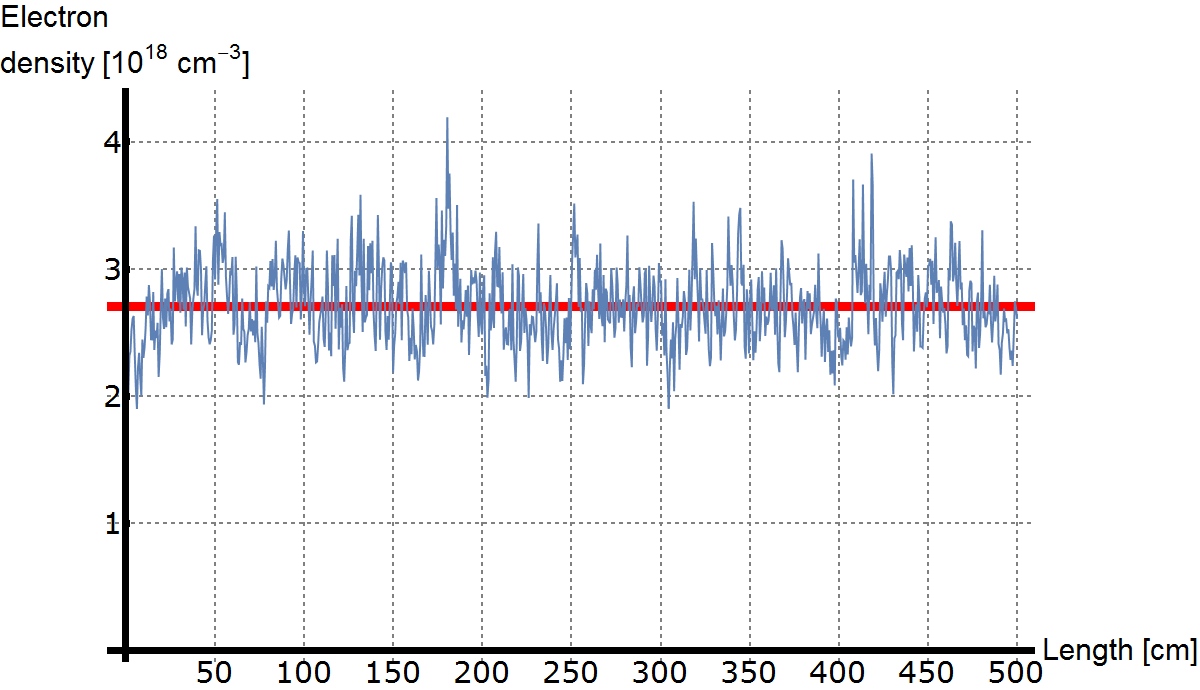
\includegraphics[width=\textwidth]{figures/spectro/longitudinal_profile.png}
    \caption{Longitudinal plasma density profile in a \SI{5}{\cm} long, \SI{0.5}{\mm} diameter straight capillary. Red line indicates average density.}
    \label{fig:longi_profile}
\end{figure}


\section{Two stage capillary}
As stated in the theoretical introduction (section \ref{sec:wakefield}), a "fish--bone" capillary composed of two channels or more can be used to overcome limitations in the dephasing length when accelerating electrons. For that goal we designed a Y--shape capillary (figure \ref{fig:doublecapillaryCAD}) on which we performed an experiment to investigate the parameters that permits optical guiding in a very similar way to that presented in section \ref{sec:duration-of-guiding}.
\begin{figure*}
    \centering
    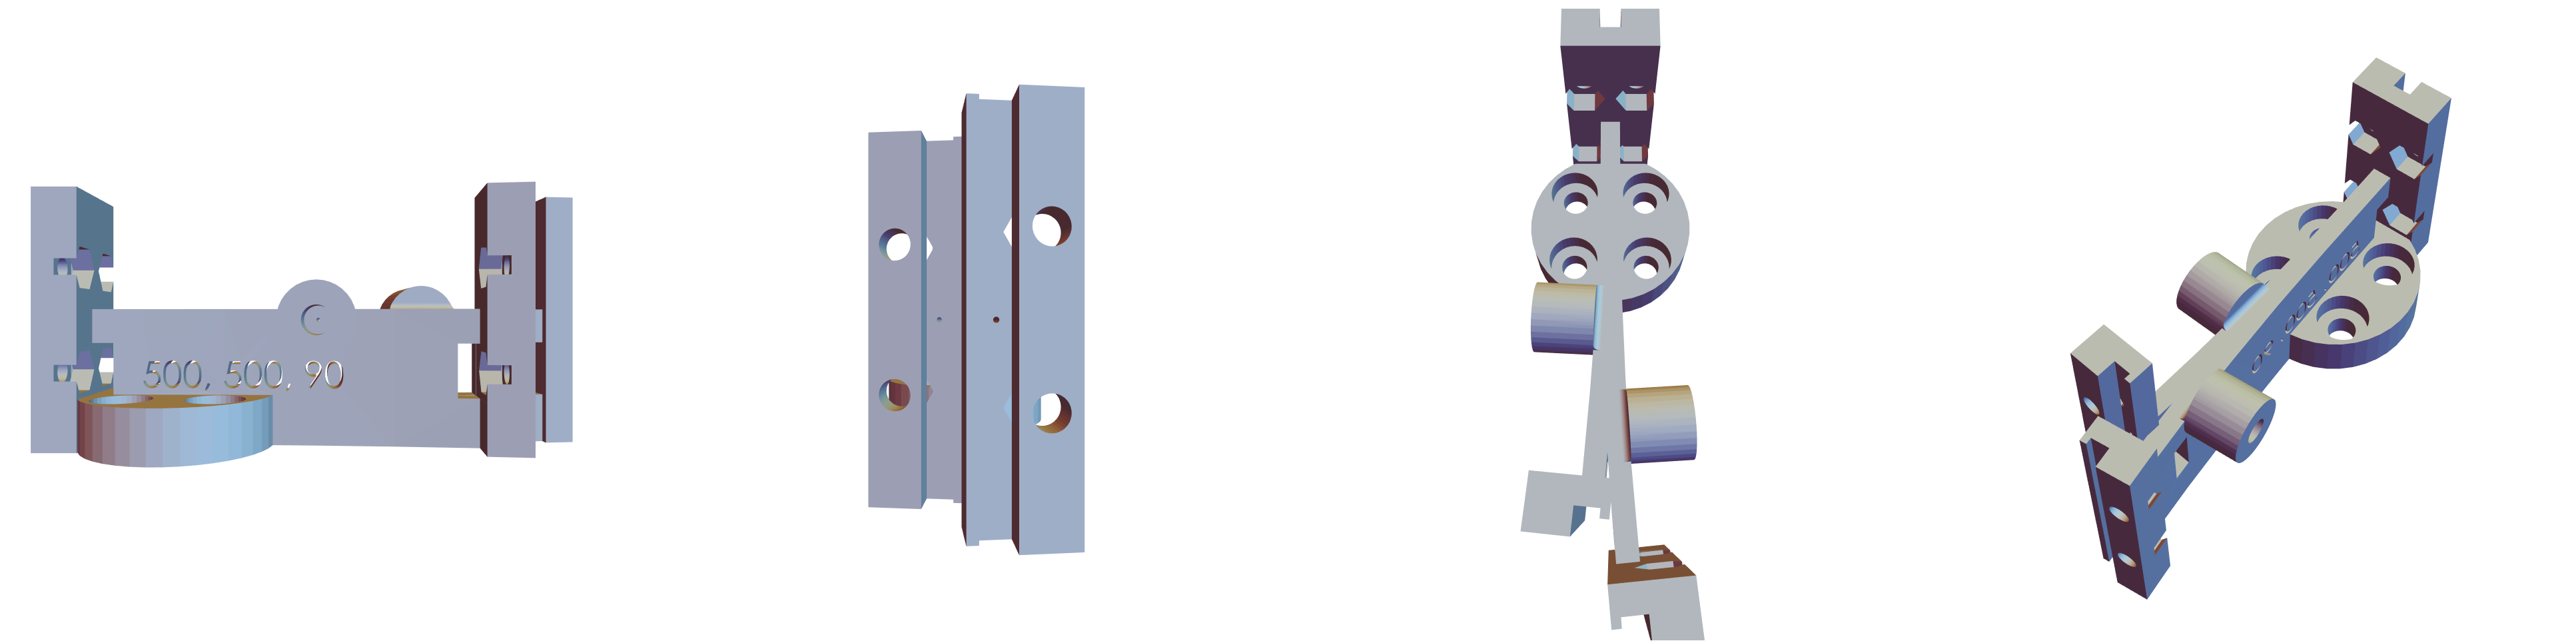
\includegraphics[width=\textwidth]{figures/cad/doublecapillary_cad.png}
    \caption{3D drawing of the 2--stage capillary. Designed by Yair Ferber.}
    \label{fig:doublecapillaryCAD}
\end{figure*}

The proposed method is to split the oscillator pulse--train into two beams, one for each capillary channel. In order to differentiate between the two when viewed on an oscilloscope, one beam entered a \SI{6}{\ns} delay line, resulting the temporal profile shown in figure \ref{fig:oscillator_double}. As before, a fast--photodiode was mounted outside the vacuum chamber, collecting the light from the two beams after passing through the channels.
\begin{marginfigure}
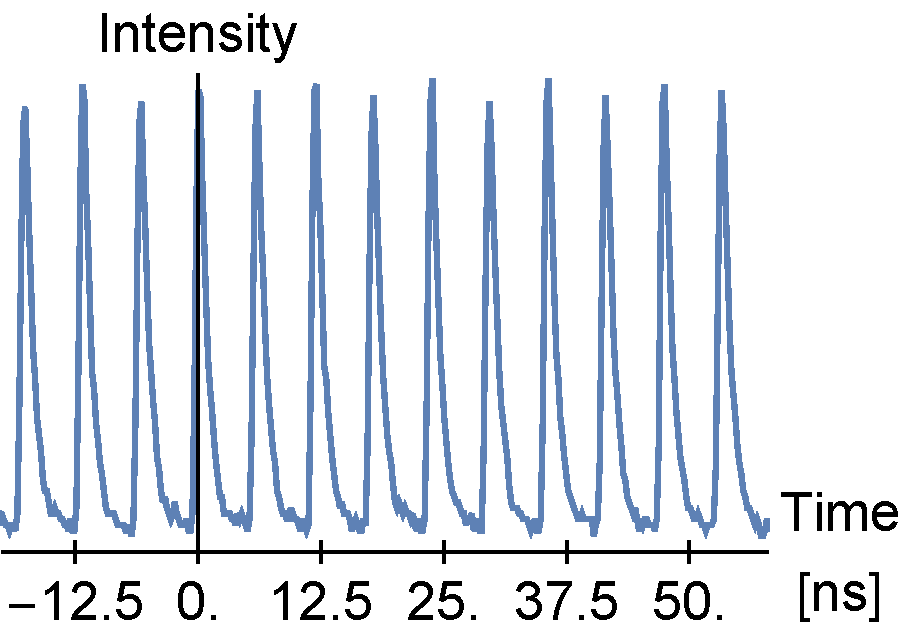
\includegraphics[width=\marginparwidth]{figures/oscillator/double.pdf}
\label{fig:oscillator_double}
\caption{Two \SI{84}{\MHz} temporal beam profiles of the oscillator laser, one delayed with respect to the other.}
\end{marginfigure}

The two channel capillary goes a step beyond the straight one, but complicates the measurement in a few aspects. Note that the curved channel doesn't posses a line--of--sight from the entrance plane to the exit plane; The capillary radius of curvature (\SI{50}{\cm}), \textcolor{red}{length} (\SI{5}{\cm}) and diameter (\SI{500}{\um}) doesn't allow a straight ray to propagate through it --- see figure \ref{fig:lineofsight}. For that reason, when carefully aligning the laser beam, we relied on refractions from the capillary plastic walls to be collected and focused by a positive lens outward to the photo--diode.

As a first check, we performed the measurement only on one channel, the shorter of the two. We inserted a metal wire to the longer one, thus dis--functioning it by blocking plasma from entering it.

\begin{figure}
    \centering
    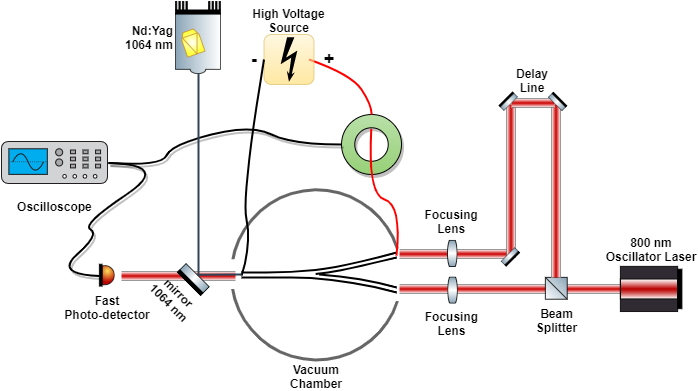
\includegraphics[width=\textwidth]{figures/Curved capillaries/system double capillary.png}
    \caption{Experimental system for the Y--shape, curved capillaries.}
    \label{fig:twostage_system}
\end{figure}

In contrast to the previously presented measurements, now a stable, jitter controlled operation was achieved when the triggering Nd:Yag laser pulse was delivered to the \textbf{positive} electrode, as opposed to the set--up until now, in which it was delivered to the negative one. The inverse arrangement also caused electromagnetic noise to the surrounding, which, in turn affected the recorded signal of the measuring devices (Rogowsky coil and photo--detector).

We estimate the jitter to be very similar as that obtained in section \ref{sec:jitter}, at $\tau_\text{jitter}\approx 6\pm 1\si{\ns}$.

\begin{figure}
    \centering
    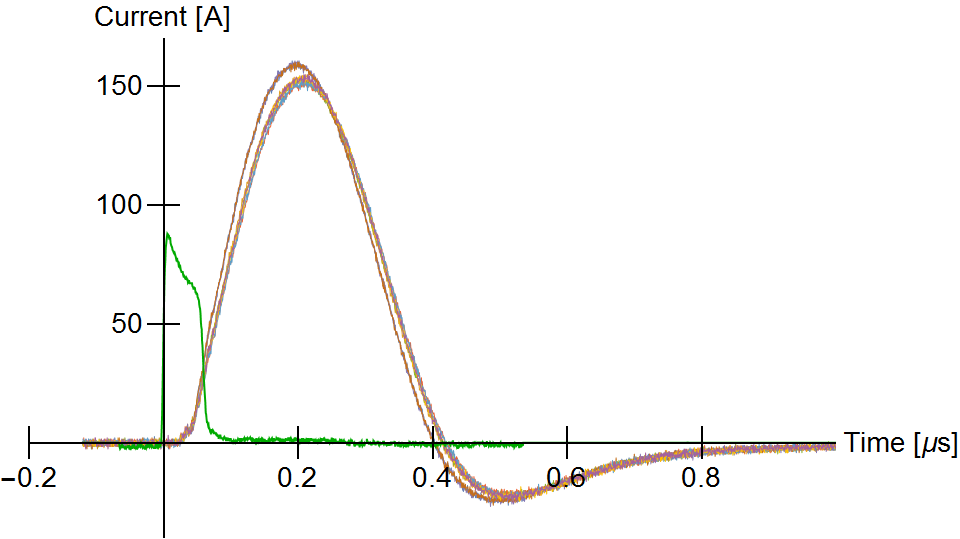
\includegraphics[width=\textwidth]{figures/Curved capillaries/low_jitter_curved_capillary.png}
    \caption{Caption}
    \label{fig:Demonstration of low-jitter ignition set--up when generating plasma in the curved capillary. A plot of nine consecutive Rogowsky coil current profiles in reference to the igniting Nd:Yag pulse (Green).}
\end{figure}

\begin{marginfigure}
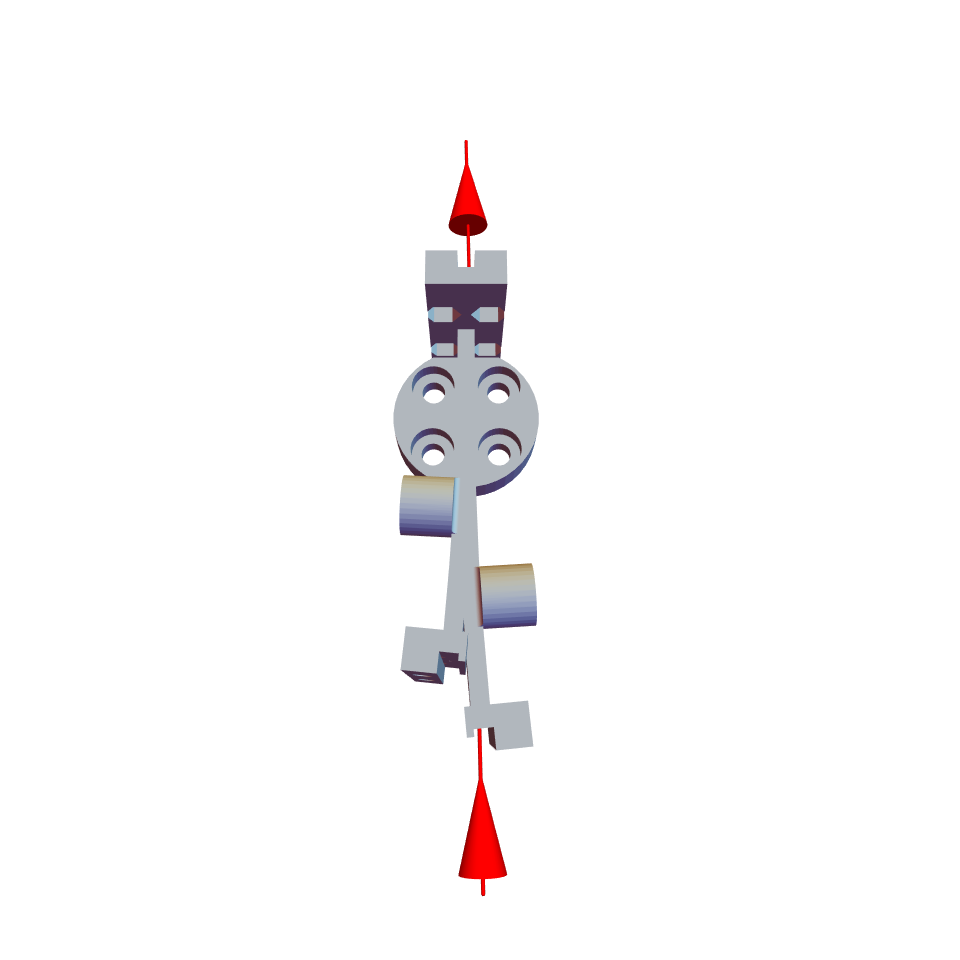
\includegraphics[width=\marginparwidth]{figures/Curved capillaries/line-of-sight.png}
\caption{The curved channel does not posses line--of--sight.}
\label{fig:lineofsight}
\end{marginfigure}

Another thing to point out, is that when creating a plasma discharge, the photo--diode also detected unwanted light from the emitting plasma --- light that is collected by the same lens that focuses the oscillator laser. This plasma light caused a "bump" in the time--domain voltage profile monitored on the oscilloscope, with a maximal peak of about 7 to 8 that of the oscillator signal prior to the plasma discharge. To minimize this effect we positioned an opaque screen with a small hole (about \SI{1}{\mm} in diameter) in the capillary exit plane (figure \ref{fig:opaque}).

\begin{marginfigure}
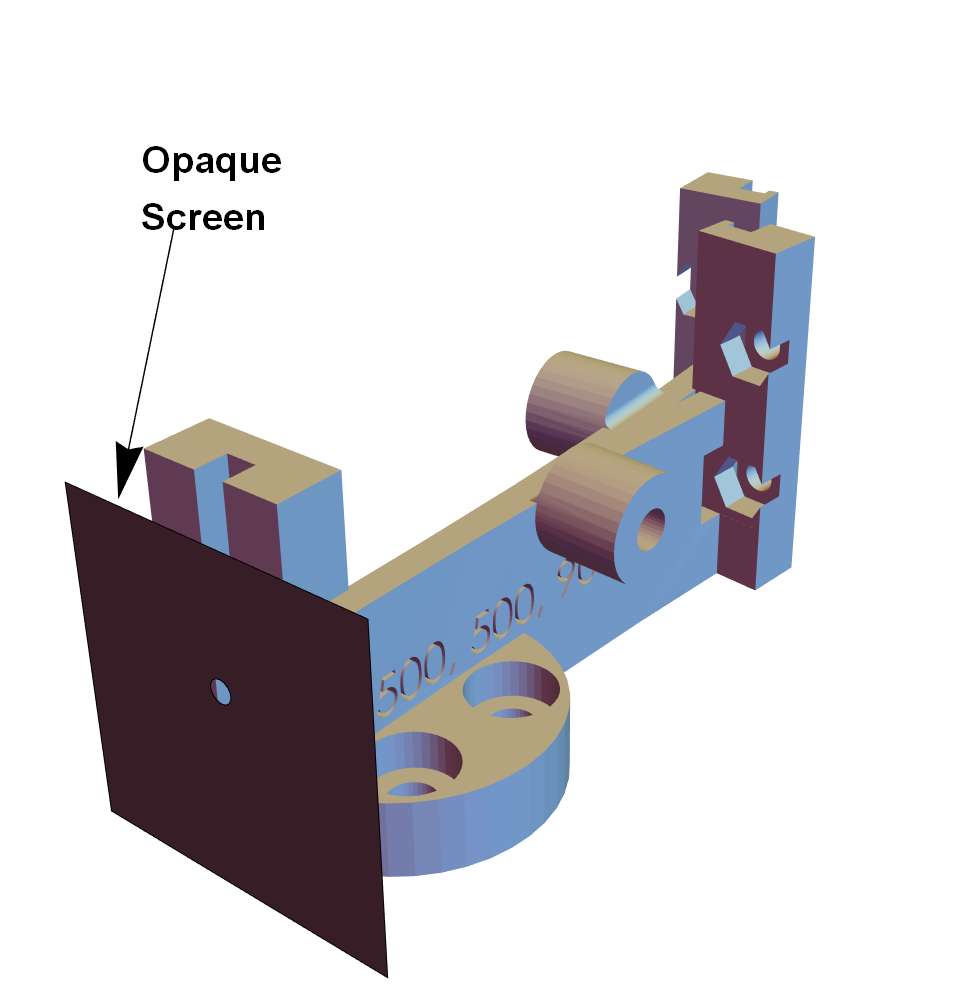
\includegraphics[width=\marginparwidth]{figures/cad/opaquescreen.png}
\caption{Opaque screen with a small hole positioned close to the back plane of the capillary, intended to block light emitted from the plasma discharge.}
\label{fig:opaque}
\end{marginfigure}

Unfortunately, at the time of writing and the assignment due, we did not manage to observe a plasma channel and optical guiding.
%The following results are not ideal, but show the
Figures \ref{fig:bump-longwindow}-\ref{fig:bump-shortwindow} demonstrate a single capillary discharge in a curved channel. The plasma discharge is timed with the igniting Nd:Yag laser pulse (green waveform), and the Rogowsky coil indicates satisfactory plasma discharge. The \SI{800}{\nm} pulse-train (bottom plot) is observed prior to the Nd:Yag pulse, then sharply rising up at time $t=0$ due to scattered Nd:Yag light, and then rises up in a "bump" shape --- caused by light emitted by the plasma (minimized as much as possible by the opaque screen at the capillary front). The former was not significant in the previous measurements due to the use of a \SI{0}{\degree}--mirror for the Nd:Yag wavelength, together with the fact that pulse was delivered to the other side of the capillary, so that less scattered light reached the photo--detector. The latter, the slowly varying bump, was eliminated in the previous measurements using an aperture (iris diaphragm) positioned between the capillary and the photo--detector, before the focusing lens. We mounted a stop in the current set--up too, but that wouldn't redact completely the unwanted light.

Note that these two optic signals that the photo--detector catches are not problematic, and one is still able to infer information about the system and the plasma process. We see the decay in the transmittance (\SIrange{0.2}{1.5}{\us} after ignition), and the re--appearance of the oscillator signal after the plasma vanishes from the capillary and diffuses to the vacuum chamber. This implies that the plasma does influence the laser radiation, with the lack of conditions for transportation of the laser radiation.

At this point of the research, we conclude that, in this set--up, no plasma channel forms in the capillary discharge.

%\begin{figure}
%    \centering
%    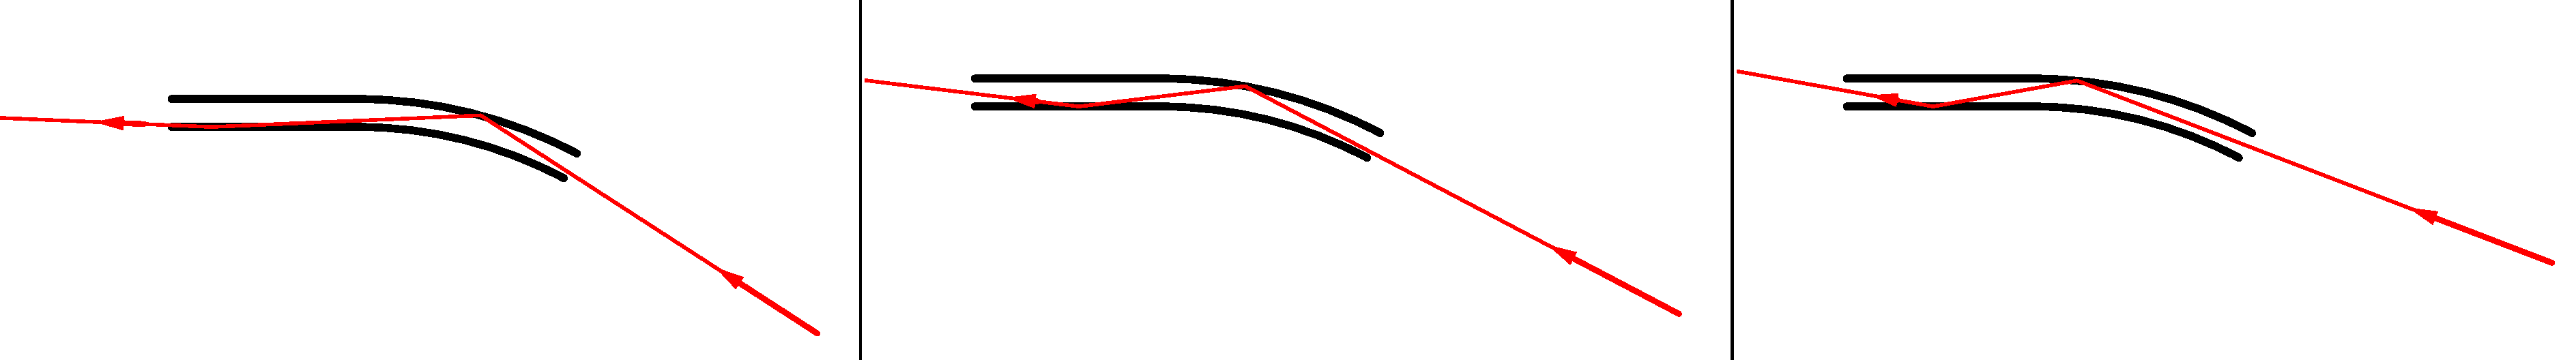
\includegraphics[width=\textwidth]{figures/Curved capillaries/inner-refractions.pdf}
%    \caption{}
%    \label{fig:my_label}
%\end{figure}
%\todo{A cartoon showing the sensitive coupling The curved channel is sensitive to the entrance vector of the guided beam.}
\begin{figure}
    \centering
    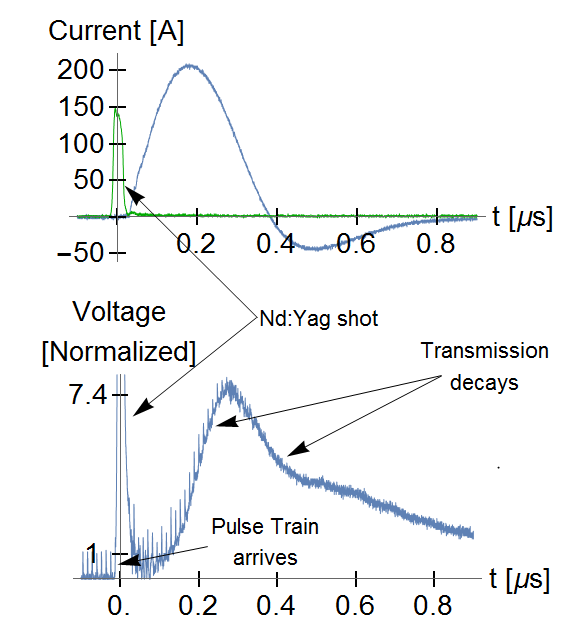
\includegraphics[width=\textwidth]{figures/Curved capillaries/curved-pulsetrain-short.png}
    \caption{Optical bumo, no guiding}
    \label{fig:bump-shortwindow}
\end{figure}
\begin{figure}
    \centering
    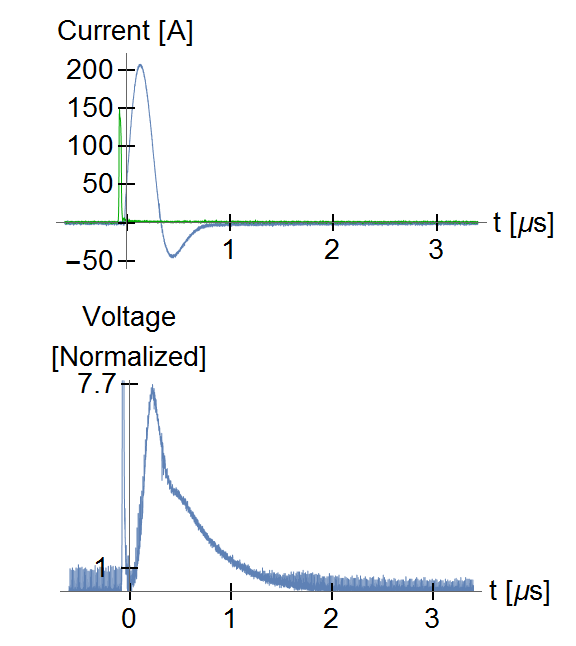
\includegraphics[width=\textwidth]{figures/Curved capillaries/curved-pulsetrain-long.png}
    \caption{Caption}
    \label{fig:bump-longwindow}
\end{figure}

\end{document}